
%% PLANUNG %% 

\chapter{Conception and Design}
This section deals with the conception of the graphical user interface and the implementation options of the application.
\section{Graphical User Interface}
First, a look is taken at whether the graphical user interface plays an important role in applications at all. For this purpose, a question on this topic was also included in the survey already mentioned. The answers on this question revealed that the graphical interface of an application, in fact, plays a role in terms of the trustworthiness of the application. Figure 6.1 shows the results of the survey-question.
\begin{figure}[H]
	\centering
	\includegraphics[scale=0.4]{appUiImportant.png}
	\caption[Survey Question]{Survey Question - Trustworthiness of the Application based on the UI}
\end{figure}
\noindent
Respondents of the survey were also given the opportunity to choose between three different UIs. The graphical interface should be adapted to the choice made by the people interviewed.
\subsection{Conceptual Design of the Graphical User Interface}
The UI can be designed based on the requirements analysis of the application and the information obtained from it. As already defined there, the application should be designed to be as intuitive and easy to use as possible. The implementation of the design of the user interface, for the android version, is based on suggestions from the material.io website [material.io], an open-source design system developed by google. The integration of the design components into the Flutter application is simplified thanks to the pre-installed material.dart package. This package is based on the source mentioned and currently supports version 2 of material.io. Support for the current version 3 of Material Design is still being worked on.
\noindent
One goal of this application is to be designed to be intuitive. In his book "UI is COMMUNICATION", Everett N. McKay described an intuitive UI as follows: 
\begin{quote}
	\textit{"A UI is intuitive when target users understand its behavior and effect without use of reason, memorization, experimentation, assitance, or training."} - Everett N McKay [Quelle]
\end{quote}
In order to meet this definition, goals that the user interface should meet could be set before the graphic user interface is designed.\\
\noindent
On the one hand, the user should be able to recognize immediately that a component of the screen is a widget that he can operate. The system must then show the user that something has been triggered by his action. This can be done, for example, through feedback in the form of a loading circle if required data still needs to be loaded, or in the form of a new screen, pop-up or similar design components. [everett] Another step that can be taken to make the application more intuitive is the correct (short) labeling of the respective components. For example, a corresponding text, or even better imagery [ess mobile interac design cameron, seite 172], should be stored on a confirmation button. In addition, it should be ensured that surface components do not change their positions. This ensures that users can rely on their previous interactions and thus learn how to use the application. Minimalism is becoming a trend not only in the real world, but also in the digital world. This can also be seen looking at the most popular graphical interface of the survey, shown in Figure 6.2. The associated surfaces can be found in Appendix x.
\begin{figure}[H]
	\centering
	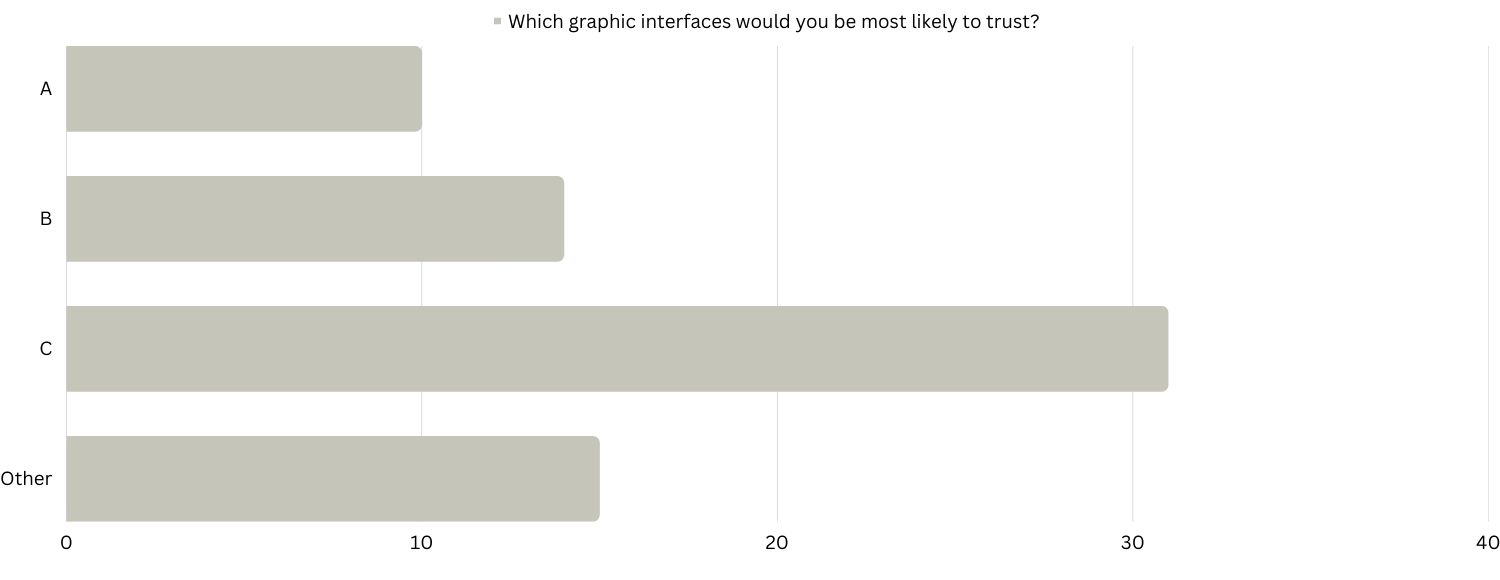
\includegraphics[scale=0.4]{whichUI.png}
	\caption[Survey Question]{Survey Question - Which UI}
\end{figure}
\noindent
Designing the application as minimalistic as possible has the advantage that the graphical interface is not overloaded and thus the user is not overwhelmed by different widgets at all. This may make it easier for the user to better interpret the use of specific elements. Another factor that plays a role in user-friendliness is to use familiar design patterns. This ensures that users are already familiar with the handling of the app elements and that there is no confusion regarding the use. 

\subsection{Description of the Views and Thoughts on the Implementation in Flutter}
This section presents the individual views that are made available to users. In addition, first thoughts on possible implementation ways for those views, working with Flutter, are considered.
\subsubsection{\textbf{Home Screen}}
The first view that a user will encounter when installing or opening the application is the home screen. There, he should be given the opportunity to switch between the different views that are necessary for his use: diagnosis creation, diagnosis overview and advice view. In addition, every user should be able to access the login screen for doctors, since they can verify themselves there as such. The navigation to create a diagnosis is implemented in the form of a button and labeled with a corresponding, clearly formulated text. To get to all other screens, a list view of all options is offered, in which there are various clickable fields that trigger navigation to the corresponding screen when clicked. In Flutter, this view can be achieved through several different components. The most important widgets can be used in the form of children in a column. In order to implement the clickable forwarding elements to other views, one should use a ListView, storing children of the widget GestureDetector, which allows any widget to be clickable. The childrens can be stored in an external modifiable list, this allows you to simplify the integration of new categories at a later point in time. A mock-up of a possible home screen can be found in Appendix x.

\subsubsection{\textbf{View for the diagnostic process}}
The screen to start a diagnosis should be designed as simple as possible. Users can adress on which body part they are feeling their symptoms. Based on their selection the application shows all symptoms associated with the body part, which then can be selected and afterwards specified by the user. The widget \textit{Stepper} is a possible implementation option. It gives the developer the opportunity to easily implement a type of step-by-step tool. For this purpose, only all steps for generating a diagnosis are created and filled with the appropriate data. The full code for an example Stepper-widget can be found in the appendix x.

%	\scriptsize
%	\begin{lstlisting}[caption=Stepper for Body Part Selection]
%		...
%		  List<String> selectedBodyParts = [];
%		...
%		Stepper(
%		type: stepperType,
%		physics: ScrollPhysics(),
%		currentStep: _currentStep,
%		onStepTapped: (step) => tapped(step),
%		steps: [
%			...,
%			Step(
%				title: const Text('Location of the Symptoms'),
%				subtitle: const Text(
%				"Please select the body Part ...",),
%				title: const Text("Body Parts"),
%				onTap: (values) {
%					setState(() {
%						selectedBodyParts = values;
%					});},),
%			isActive: _currentStep >= 0,
%			state:
%			_currentStep >= 0 ? StepState.complete : StepState.disabled,
%			),
%			...
%	\end{lstlisting}
%	\normalsize
\subsubsection{\textbf{Login Screen (Doctor)}}
The login screen is displayed to the user immediately after clicking on the navigation tool labeled "Doctor Panel". There he will be offered the option to log in or register. This is achieved by simply adding editable textfields for the needed user input: email, password and confirmation password. If the user has already created a user account in a previous session, has verified himself as a medical profressional and has then been logged in, he will be forwarded to the actual doctor panel without any further need to log in. An exception is given if he has previously logged out. With the help of the flutter\_login package, a developer can implement the login process in Dart very easily. Appendix x demonstrate the use of the FlutterLogin-plugin. There are also options to customize the appeareance of the login-form.
%	\scriptsize
%\begin{lstlisting}[caption=Stepper for Body Part Selection]
%	...
%	FlutterLogin(
%		logo: const AssetImage('assets/images/login.png'),
%		title: 'Please login to continue',
%		onLogin: AuthService.instance.signIn,
%		onSignup: AuthService.instance.registration,
%		onConfirmRecover: AuthService.instance.resetPassword,
%		onSubmitAnimationCompleted: (() {
%			Navigator.of(context).pop();
%			AppNavigator.push(Routes.doctorPanel);}),
%		onRecoverPassword: (_) => Future(() => null),)
%	...
%\end{lstlisting}
%\normalsize
\subsubsection{\textbf{Screen with all body parts, diseases, advices and symptoms (Doctor)}}
The doctor panel should contain all the necessary data related to the records stored in the database. Here, a doctor can switch between the different collections. A good implementation method for this would be the BottomNavigationBar. It contains various navigation elements, which all change to their data view when you click on them. The data views show a list of the data stored in the associated Firestore collection. Care should be taken to ensure that it is recognizable that you can click on the list elements. When the user clicks on such an element, the system redirects to the edit view for the associated record. In order to be able to store new data quickly, a FloatingActionButton can also be integrated, which opens a small menu by clicking on it, where all the data add options for the doctor are listed. Clicking on a listing item then opens the associated add view.
\subsubsection{\textbf{View for adding and editing data (Doctor)}}
In order to make the views as intuitive as possible, it is advisable to make the graphical interface as uncluttered as possible. Furthermore, here only text fields are included for the data records where possible. For the selection of related data for a data set (e.g. symptoms for an illness), a button is placed on the view which, when clicked, generates and displays a dialog with the content of all symptoms in the database. Ideally, this dialog should also contain a search bar so that the user is not forced to scroll through the large number of data records. Both, the edit view and the view to add new records, consist of a form widget. In this it is possible to transfer text fields as children, which can be modified by a user. The distinction here is only between the initial value of the text fields. While the data stored in the database for the associated data record is displayed in the edit view, when a new data tuple is created, only an empty text field with a note regarding the data field is specified.
\subsubsection{\textbf{View with all saved diagnoses}}
The diagnoses view is represented by a vertical list of all diagnoses. A ListView is used here. This ListView contains all diagnostic data that the user has previously saved on his device. Clicking on a diagnosis element in the list opens the detailed view of this diagnosis. It shows the date on which the diagnosis was made, which symptoms the user specified and which illnesses resulted from the calculation of the probability of diseases. This are represented in the form of a bar chart. At the end of the diagnosis, the diseases are listed again in list form, together with their description and treatment recommendations.

\subsubsection{\textbf{View with all advices stored in the database (User) }}
The recommendation screen is laid out similarly to the diagnosis screen. Here, too, the data from Firestore is displayed in the form of a vertical list and a click opens the detailed description of the advice. This detailed view simply consists of text fields which contain the data from the document fields.
\subsection{Mock-ups and Survey regarding the Trustworthiness of Mock-up Designs}
With the description of the screens and the first development approaches, mock-ups could already be created with the help of Canva. These can be found in Appendix x. As parat of a survey, it was founrd out whether the basic idea of the graphic design would speak for trustworthiness and whether the participants woudl have inutitively known how to interact with the interface. The results are presented below.

%\section{The Symptom Graph}
%\subsection{Performance Evaluation}
%\subsection{Scalability Comparison}


\chapter{Implementation}
Based on the specifications from the previous chapter, it is now possible to open the app to implement. This chapter describes the technologies used for the development of this application. The project structure is also examined in more detail.
\section{Project Structure}
When developing software systems in the client-server, it is advised to make sure that the project and class structures are divided into three different layers.
\begin{itemize}
	\item \textbf{Data Layer}
	\newline
	The data layer takes care of retrieving the (raw) data from the database. For this purpose, a class named DatabaseService is generated as part of the Flutter application, which can be instantiated.
	\scriptsize
		\begin{lstlisting}[caption=Stepper for Body Part Selection]
		class DatabaseService {
			/* CREATE AN INSTANCE OF THE DATABASE */
			DatabaseService._();
			static DatabaseService _instance = DatabaseService._();
			static DatabaseService get instance => _instance;
		}
		\end{lstlisting}
	\normalsize
	Using DatabaseService.instance.\_methodName, each method of the service can now be called globally from anywhere in the project.
	\item \textbf{Business Logic Layer}
	\newline
	With the help of the business layer, the data that is now received from the database service can be converted into models with which the system can work accordingly. For this purpose, a ConvertService can be created similar to Listing 7.1, which can be instantiated in the same way. This now queries the data using the DatabaseService.instance and converts the data which is supplied by the Firestore API in the form of DocumentSnapshots, Streams or QuerySnapshots. The data models for this are presented in the Data Models section.
	\item \textbf{Presentation Layer}
	\newline
	This layer takes care of mapping the data to the graphical interface. To do this, it queries the model data of the ConvertService and creates the widgets that are to be displayed accordingly.
\end{itemize}
In project development, it is increasingly interesting how applications receive their data. As part of this work, this will happen through API queries to the Firestore database. The whole procedure is also known as the client-server model. An example of the communication process, together with the services that just got described, is shown in Figure 7.1. 
\begin{figure}[H]
	\centering
	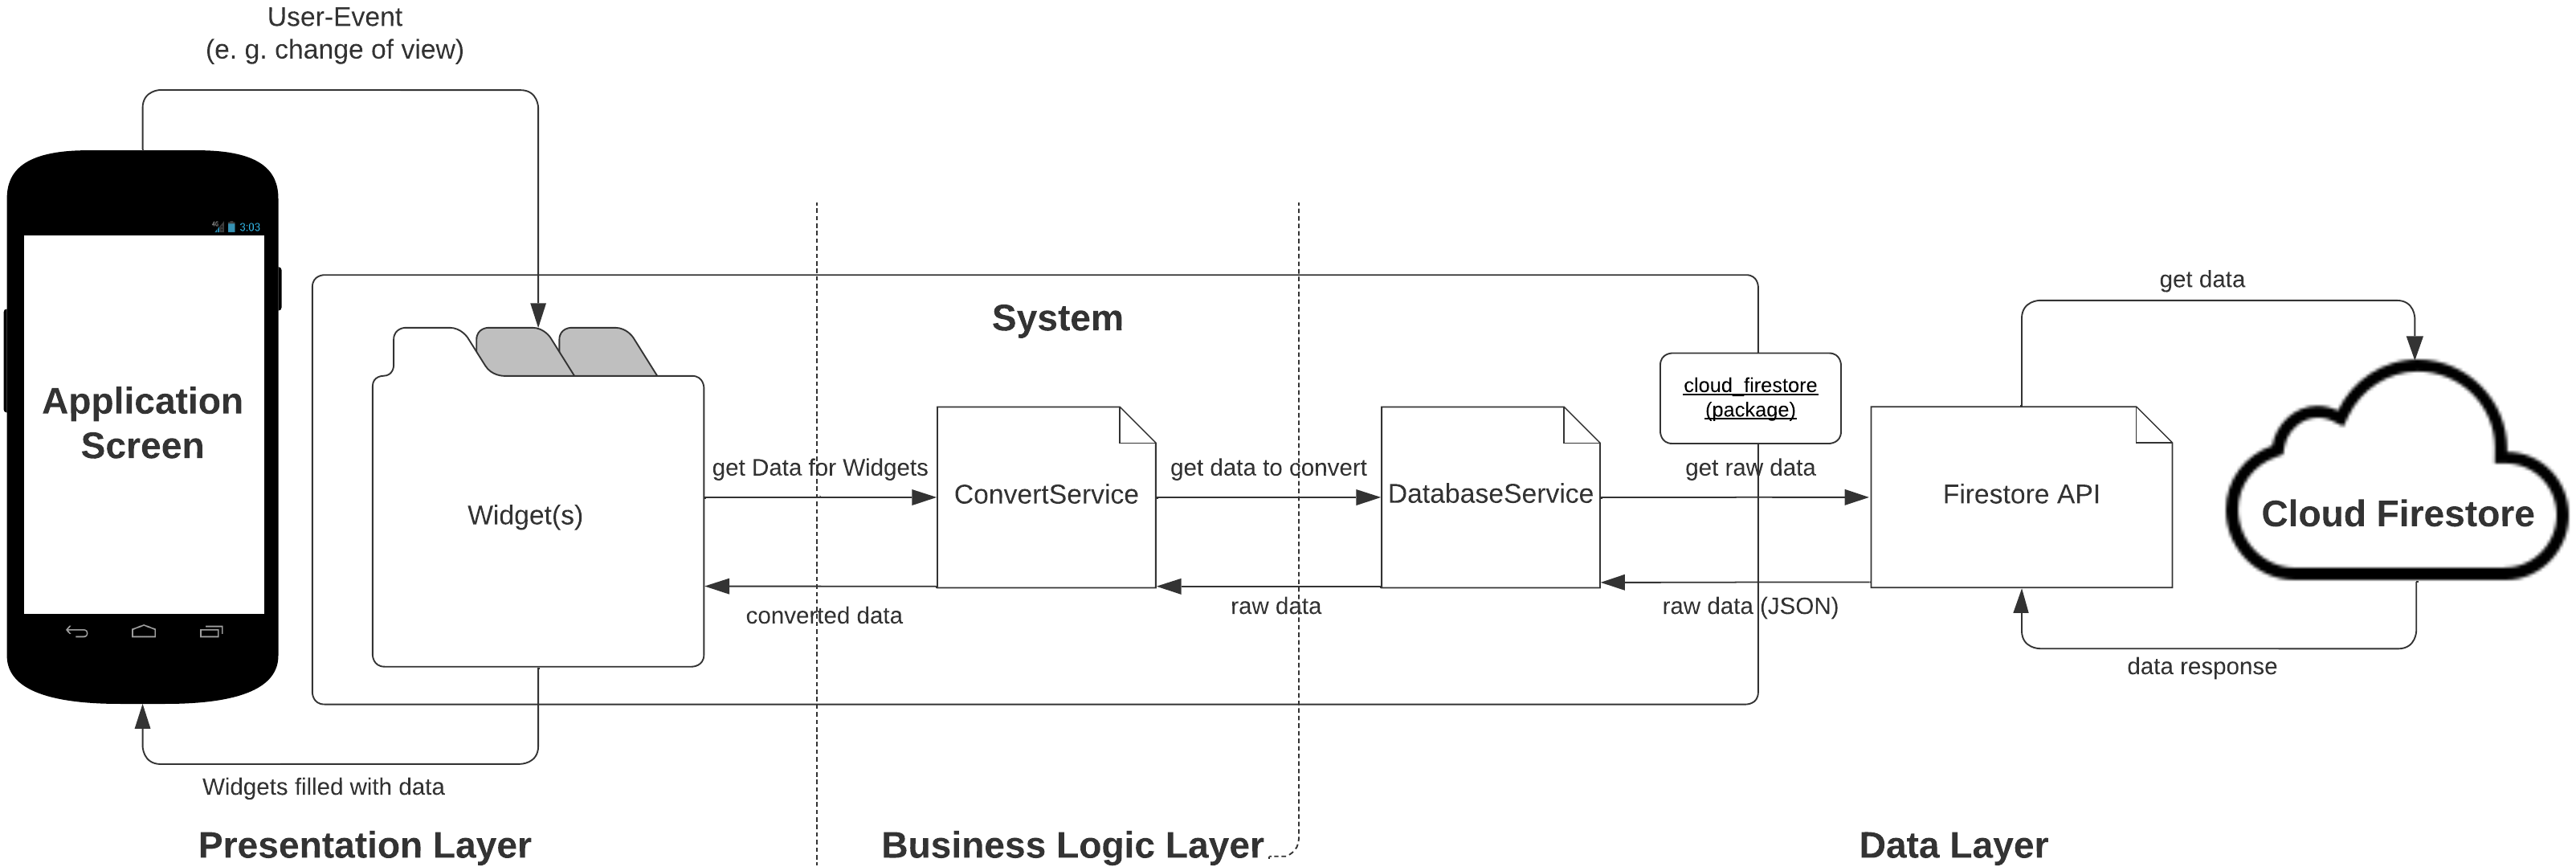
\includegraphics[scale=0.2]{api_flow.png}
	\caption[Client-Server Request Flow]{Client-Server Request Flow}
\end{figure}
\noindent
\subsection{Routing in the Application}
Another step that can be taken to keep the project structure as clean as possible is to lay out the navigation in an extra class. In this work, a class that is named AppNavigator is created for this purpose. This navigator can then be called globally using a defined method AppNavigator.push(Route pRoute). The route parameter is an element of an enumeration which refers to different views of the application. All AppNavigator code can be found in Appendix x.
\section{Data Models}
The data model into which the ConvertService converts the raw data of the DataService is based on the document structure stored in the database. When scraping the data of the JSON responses, the data is converted as follows: String$\,\to\,$String, Array$\,\to\,$List, Map<key, value>$\,\to\,$Map<String, dynamic>, Number$\,\to\,$num. Listing 7.2 shows the resulting model for symptoms. All other Models can be found in the appendix x.
\scriptsize
\begin{lstlisting}[caption=Model for Symptoms]
class Symptom {
	final String? id;
	String name;
	List<String> symptoms;
	
	Symptom({this.id, required this.name, required this.symptoms});
	
	Map<String, dynamic> toMap() {
		return {
			'name': name,
			'proposed_symptoms': List<String>.from(
			symptoms.map((x) => x),
			),};}
	
	Symptom.fromDocumentSnapshot(DocumentSnapshot<Map<String, dynamic>> doc)
		: id = doc.id,
		name = doc.data()!["name"],
		symptoms = List<String>.from(
		doc.data()!["proposed_symptoms"].toList(),);	
}
\end{lstlisting}
\normalsize


\section{Algorithms for the Attribution of Symptoms to potential Diseases}
\subsection{List Matching}
Die erste Methodik welche betrachtet werden soll basiert auf rein theoretischen Aspekten. Durch Angabe der vom Patienten angegebenen Symptome setzt die Applikation eine Liste von diesen zusammen. Währenddessen konnte man bei dem Befüllen der Datenbank mit den nötigen Datensätzen feststellen, dass für jede Krankheit ebenfalls eine Liste an Symptomen hinterlegt wird. Eine intuitive Idee wäre, diese beiden Listen miteinander zu vergleichen entsprechend dazu einen Matching-algorithmus zu entwickeln, welcher die prozentuale Übereinstimmung der Listen kalkuliert. Das sogenannte Word-Matching wird in Quelle [] beschrieben. Bei diesem vorgehen sollte jedoch beachtet werden, dass keinerlei medizinische Daten bei der Berechnung mit einfließen. Dementsprechend sinkt die Wahrscheinlichkeit der Korrektheit der Diagnosestellung. Im Sinne dessen soll eine weitere, genauere Methode betrachtet werden.

\subsection{Bayesian Networks}
Entsprechend der fehlenden Genauigkeit der eben definierten Methode wird nun ein genaueres Verfahren betrachtet. Ein sogenanntes Bayesian Network stellt einen Wahrscheinlichkeitsmodel in Form eines directed acyclic graphs (DAG) auf. \cite{.bahn-bonn}
\subsubsection{Directed Acyclic Graphs}

\subsection{Algorithmische Lösung mit Gewichtungen}
Zunächst wird die im conference paper "towards a ranking of likely diseases in terms of precision and recall" beschriebene Symptomzuordnung untersucht. Das Dokument wurde zwar schon im Jahr 2012 veröffentlicht, geht aber auf Problematiken ein, welche auch heute noch bei bestimmten Krankheitszuordnungsverfahren vorhanden sind und eine, mit Medizinern erarbeitete, Lösung, wie diese Verfahren sauber ersetzt werden können. Die Informationen welche aus dem Paper entnommen werden können bieten auch heute noch eine gute Grundlage für eine algorithmische Lösung der Krankheitsermittlung.

\subsubsection{Die Einflussfaktoren der Diagnosestellung}
Zunächst werden die Einflussfaktoren betrachtet und im Rahmen der Applikation zugeordnet.
\begin{itemize}
	\item \textbf{Einteilung der Symptome}
	\newline
	Nachdem der Nutzer in der Applikation seine Symptome angegeben hat können, basierend auf den Angaben, zugehörige Krankheiten aus der Datenbank gefiltert werden. Dadurch werden alle möglichen Symptome der Krankheiten geliefert und es können zwei Mengen gebildet werden: vorhandene und abwesende Symptome. Mit Hilfe dieser Informationen wird im späteren Verlauf die Wahrscheinlichkeit einer Krankheit basierend auf den Patientensymptomen ermittelt.

	\item \textbf{Wahrscheinlichkeit des Eintretens einer bestimmten Krankheit}
	\newline
	Für die Wahrscheinlichkeit des Eintretens einer Krankheit werden im Rahmen dieser Arbeit Dummy-Daten verwendet. Das Vorgehen um diese Daten in der Datenbank zu hinterlegen wird im JupyterNotebook durchgeführt, welches wie schon beschrieben im Anhang x zu finden ist. 
	
	Zusätzlich zu dieser Information wird die Wahrscheinlichkeit benötigt, wie schwerwiegend ein Symptom tatsächlich ist. Im Paper wird dieser Wert als default importance beschrieben. Der Faktor wird ebenfalls in Form von Dummydaten hinterlegt.
	
	\item \textbf{Patientenspezifische Faktoren}
	\newline
	Zu den Patientenspezifischen Faktoren gehören Eigenschaften wie das Alter, Geschlecht oder ob der Patient raucht oder nicht. Eine Abfrage dieser Faktoren kann während der Symptomangabe erfolgen. Im Rahmen der Implementierung des Algorithmus bei dieser Arbeit werden diese Faktoren jedoch außen vor gelassen.
	
	Zusätzlich zu diesen Faktoren müssen auch der Auftrittszeitpunkt eines Symptoms und die Intensität mit welcher ein Patient dieses Symptom empfindet eingebunden werden. Diese Informationen werden im Rahmen der Symptomangabe vom Nutzer mitangegeben und temporär, in Form eines user specified symptoms, gespeichert. Die Faktoren der Itensität und Neuartigkeit sind mittels enumerationen im Programmcode hinterlegt. 
	
	\item \textbf{Relation of Diseases and Symptoms}
	\newline
	Zur Berechnung der relatedness wird zum einen die Berechnung der bedingten Wahrscheinlichkeit P(s|d) eines Symptomes und einer Krankheit benötigt und zum Anderen der Faktor, ob es sich beim Symptom um ein leitendes Symptom der Krankheit handelt. 
	
	\item \textbf{Symptom spezific factors}
	\newline
	Zur Berechnung der relatedness wird zum einen die Berechnung der bedingten Wahrscheinlichkeit P(s|d) eines Symptomes und einer Krankheit benötigt und zum Anderen der Faktor, ob es sich beim Symptom um ein leitendes Symptom der Krankheit handelt. Die Implementierung in dieser Arbeit ermittelt den Faktor, ob es sich um ein leitendes Symptom handelt ebenfalls, basierend auf dummydaten.
\end{itemize}
\noindent
Mittels der beschriebenen Faktoren können folgend die Werte precision und recall ermittelt werden. [quelle, seite 9]. Mit Hilfe dieser wiederum kann in einem weiteren Schritt bestimmt werden, in welchem Grad die Symptome des Patienten auf die Krankheitssymptome abgebildet werden können. Final lässt sich das Ranking der Krankheiten wie folgt berechnen:
\begin{equation}
	  \begin{aligned}
		r(d) := F(d) + \lambda + P_p(d)\\
	 \end{aligned}\qquad\text{aus []}
\end{equation}
Der Lambawert dient zur verminderung des Krankheitswahrscheinlichkeitwertes, da dieser laut den Autoren als weniger wichtig angesehen wird. 
\newline
\noindent
Das Paper geht unter anderem auf Problematiken welche bayesian networks mit sich bringen ein: viele wichtige Faktoren welche für die korrekte Berechnung der Symptomwahrscheinlichkeiten nötig sind, sind quasi unzugänglich und unbekannt. 

\subsection{Machine Learning}
%[13]. Since Bayes-nets are
%theoretically best suited for diagnosis they are successfully implemented in some
%of the mentioned expert-systems. However statistical approaches like Bayes-nets
%require knowledge, which isn't broadly available: e.g. the a-priori probabilities for
%signs and symptoms P(s) are mostly not known. Thus we are not able to compute
%the conditional probability for a disease, given the symptom P(djs) = P(sjd)P(d)
%P(s)
%with the help of Bayes-Theorem. Note that P(sj:d) is normally not known as
%well. It is not dicult to see that even though we cannot calculate P(d1js) and
%P(d2js) for two diseases d1 and d2, we are able to compare them by computing
%P(d1js)=P(d2js). Thus, without knowing P(s), ranking diseases is possible.
%Similar to our approach is the work described in [14], where a quality measure
%for diagnosis is dened. However the factors inuencing the ranking are dierent
%(e.g. they assume to have knowledge about the probability of a nding being
%caused by a certain disease). Further they do not allow the clinicians to interact
%with the system and change e.g. symptom weights. In [15] a model similar to
%ours represents the disease-symptom relations using fuzzy labels, however the
%symptoms itself are not weighted. They also chose an IR approach to rank likely
%diseases.
\subsubsection{Naive Bayes (Classifier)}
Ein Klassifikator macht es möglich, Eingabedaten einer bestimmten Klasse zuzordnen. Sie werden besonders oft im Machine Learning bereich eingesetzt, beispielsweise für die Erkennung vom Spammails. Im Rahmen der Symptomanalyse wird einem hier ermöglicht, Eingabedaten in Form von Symptomen auf bestimmte Krankheitsklassifikationen abzubilden. [quelle unicamp.br] Das Gesamtergebnis der Berechnung ergibt dann die bedingte Wahrscheinlichkeit des Symptoms basierend auf den Eintrittswahrscheinlichkeit der Symptome zu den Krankheiten. 
\section{Evaluation of the Algorithms}
\section{Diagnoses}
\subsection{Generate Diagnose PDF}
\subsection{Store PDF Locally on Device}
